\section{Search for same-sign dileptons with $b$ jets}
\label{searchbtag}

This analysis is based on the inclusive same-sign dilepton search documented in AN-2011/258~\cite{ssnote2011} and corresponds to an
integrated luminosity of 349 pb$^{-1}$. In that study we searched for events with two isolated same-sign leptons
in association with 2 additional jets and \met. Here we re-use most of the baseline event selection~\footnote{The additional 
$Z$ veto is not applied in this study}. In addition, we require at least 2 b-tagged jets using Track Counting High Efficiency 
Medium (TCHEM) working point tagger~\cite{BTVPAS2011}. We refer to TCHEM with the requirement that three of the tracks have $IP$ 
significance $ > 3.3$. For this tagger the b-tagging efficiency is $0.62 \pm 0.01$ and the acceptance of light flavor jets 
is $0.018 \pm 0.004$~\cite{BTVPAS2011}.

\subsection{Event Selection}
\label{eventsel}

The event selection for high p$_T$  and low p$_T$ baseline regions are briefly summerized as follows:

\begin{itemize}
\item At least two isolated same-sign leptons ($ee$, $e\mu$, and $\mu\mu$) with $|\eta| < 2.4$
\begin{itemize}
\item For the high-$p_T$ study, both leptons are required to be $p_T > 10$ GeV, with one of them $p_T > 20$ GeV.
\item For the low-$p_T$ study, the electrons are required to be $p_T > 10$ GeV and muons $p_T > 5$ GeV.
\end{itemize}
\item At least two particle flow jets tagged using TCHEM tagger with $p_T > 40$ GeV and $|\eta| < 2.4$ corrected with L1FastL2L3 corrections.
\item The selected jets must be separated from the lepton by $\Delta R > 0.4$.
\item The scalar sum of momenta $H_T > 80$ ($H_T > 200$) GeV is required for high-$p_T$ (low-$p_T$) analysis.
\item \met $> 30$ GeV.
\item We remove dilepton events with invariant mass $M_{ll} < 5$ GeV.
\end{itemize}

More details are found in Reference~\cite{ssnote2011}.

\subsection{Event Yields and Background Estimation}
\label{eventsel}

The results of this search in the above-mentioned kinematical region are summerized in Table~\ref{tab:ssyields1},~\ref{tab:ssyields2}. Data-driven background 
predictions are used to estimate SM backgrounds. This is based on a combination of estimating ``Tight-To-Loose ratio'' (Fake Rate)
and electron charge mis-reconstruction rate (Charge Flip rate). The probability for muons to be reconstructed 
with the wrong sign in the relevant momemtum range is negligible.

The event yields have the following characteristics:

\begin{itemize}
\item The contributions from rare processes such as $qqW^\pm W^\pm, WWW, t\bar{t}W$, and double parton $W^\pm W^\pm$ are negligibly small.
\item The diboson backgrounds $WW, WZ$, and $ZZ$ are found to be negligible.
\item The prediction from fake rates includes the systematic error of 50\%.
\item The prediction from flip rates incldues the systematic error of 25\%.
\item The systematic errors are added when propagting the fake/flip rates into the total prediction.
\item We do not consider any MC driven estimation for the final prediction.
\end{itemize}

\vspace{6 mm}
\begin{table}[htb]
\begin{center}
\begin{tabular}{|c|c|c|c|c|}
\hline
Sample & $e^{\pm}e^{\pm}$    & $\mu^{\pm}\mu^{\pm}$ & $e^{\pm}\mu^{\pm}$      & total \\ \hline
% all the MCs
\hline
\ttbar\  & 0.15 $\pm$ 0.09 & 0.25 $\pm$ 0.11 & 0.25 $\pm$ 0.11 & 0.65 $\pm$ 0.18 \\ 
Single top  & 0.02 $\pm$ 0.02 & 0.02 $\pm$ 0.02 & 0.02 $\pm$ 0.01 & 0.06 $\pm$ 0.03 \\ 
wjets  & 0.00 $\pm$ 0.00 & 0.00 $\pm$ 0.00 & 0.00 $\pm$ 0.00 & 0.00 $\pm$ 0.00 \\ 
DY  & 0.00 $\pm$ 0.00 & 0.00 $\pm$ 0.00 & 0.00 $\pm$ 0.00 & 0.00 $\pm$ 0.00 \\ 
VV  & 0.00 $\pm$ 0.00 & 0.00 $\pm$ 0.00 & 0.00 $\pm$ 0.00 & 0.00 $\pm$ 0.00 \\ 
\hline
Total MC  & 0.17 $\pm$ 0.09 & 0.27 $\pm$ 0.11 & 0.27 $\pm$ 0.11 & 0.71 $\pm$ 0.18 \\
\hline\hline
data  (349 pb$^{-1}$)     & 1  &  1  & 0  & 2      \\ \hline
fake rate prediction & & & & \\ \hline
single fake   & 0.38 $\pm$ 0.38 & 0.52 $\pm$ 0.37 & 0.00 $\pm$ 0.00 & 0.90 $\pm$ 0.52 (3 evts) \\
double fake   & 0.00 $\pm$ 0.00 & 0.00 $\pm$ 0.00 & 0.00 $\pm$ 0.00 & 0.00 $\pm$ 0.31 (0 evts) \\
fake prediction & 0.38 $\pm$ 0.38 & 0.52 $\pm$ 0.37 & 0.00 $\pm$ 0.00 & 0.90 $\pm$ 0.60 \\
\hline\hline
flip rate prediction & $0.05 \pm 0.01$ & 0 & $0.06\pm 0.02$ & $0.11\pm 0.03$ \\ \hline
total fake rate prediction & $0.38 \pm 0.43$ & $0.52\pm 0.45$ & $0.00 \pm 0.00$ & $0.90 \pm 0.69$ \\ \hline
total bkg prediction & $0.43\pm 0.43$ & $0.52 \pm 0.45$ & $0.06 \pm 0.2$ & $1.01\pm 0.75$ \\\hline
\end{tabular}
\caption{\protect Data and Monte Carlo yields for the same-sign high-$p_T$ dileptons with $H_T > 80$ GeV and \met $> 30$ GeV. Uncertainties in 
the lower three rows also include the systematic uncertanities on the method used.\label{tab:ssyields1} }
\end{center}
\end{table}

\vspace{6 mm}
\begin{table}[htb]
\begin{center}
\begin{tabular}{|c|c|c|c|c|}
\hline
Sample & $e^{\pm}e^{\pm}$    & $\mu^{\pm}\mu^{\pm}$ & $e^{\pm}\mu^{\pm}$      & total \\ \hline
% all the MCs
\hline
\ttbar\  & 0.15 $\pm$ 0.09 & 0.25 $\pm$ 0.11 & 0.30 $\pm$ 0.19 & 0.70 $\pm$ 0.19 \\ 
Single top  & 0.02 $\pm$ 0.02 & 0.02 $\pm$ 0.02 & 0.02 $\pm$ 0.01 & 0.06 $\pm$ 0.03 \\ 
wjets  & 0.00 $\pm$ 0.00 & 0.00 $\pm$ 0.00 & 0.00 $\pm$ 0.00 & 0.00 $\pm$ 0.00 \\ 
DY  & 0.00 $\pm$ 0.00 & 0.00 $\pm$ 0.00 & 0.00 $\pm$ 0.00 & 0.00 $\pm$ 0.00 \\ 
VV  & 0.00 $\pm$ 0.00 & 0.00 $\pm$ 0.00 & 0.00 $\pm$ 0.00 & 0.00 $\pm$ 0.00 \\ 
\hline
Total MC  & 0.17 $\pm$ 0.09 & 0.27 $\pm$ 0.11 & 0.32 $\pm$ 0.19 & 0.76 $\pm$ 0.19 \\
\hline\hline
data  (349 pb$^{-1}$)     & 0  &  1  & 0  & 1      \\ \hline
fake rate prediction & & & & \\ \hline
single fake   & 0.00 $\pm$ 0.00 & 0.00 $\pm$ 0.00 & 0.00 $\pm$ 0.00 & 0.00 $\pm$ 0.56 (0 evts) \\
double fake   & 0.00 $\pm$ 0.00 & 0.51 $\pm$ 0.30 & 0.00 $\pm$ 0.00 & 0.51 $\pm$ 0.30 (3 evts) \\
fake prediction & 0.00 $\pm$ 0.00 & 0.51 $\pm$ 0.30 & 0.00 $\pm$ 0.00 & 0.51 $\pm$ 0.63 \\
\hline\hline
flip rate prediction & $0.01 \pm 0.004$ & 0 & $0.02\pm 0.006$ & $0.03\pm 0.01$ \\ \hline
total fake rate prediction & $0.00 \pm 0.00$ & $0.51\pm 0.68$ & $0.00 \pm 0.00$ & $0.51 \pm 0.68$ \\ \hline
total bkg prediction & $0.01\pm 0.004$ & $0.51 \pm 0.68$ & $0.02 \pm 0.006$ & $0.54 \pm 0.68$ \\\hline
\end{tabular}
\caption{\protect Data and Monte Carlo yields for the same-sign low-$p_T$ dileptons with $H_T > 200$ GeV and \met $> 30$ GeV. Uncertainties in 
the lower three rows also include the systematic uncertanities on the method used.\label{tab:ssyields2} }
\end{center}
\end{table}

The dominant SM contribution in both low- and high-$p_T$ selections are found to be from \ttbar\ decays. The estimation
is in a good agreement with the observation. We also note that the backgrounds with respect to the inclusive same sign
dilepton search is suppressed by an order of magnitude due to the b-tag requirements.

\subsection{Discussion of Backgrounds}
\label{bkgdiscussion}

As shown earlier, the primary source of background events are from \ttbar\ decays, which are estimated using the fake rate method. Here we further investigate 
by performing a closure test on a large \ttbar\ sample~\footnote{The POWHEG sample TTToLNu2Q2B\_7TeV-powheg-pythia6\_Spring11-PU\_S1\_START311\_V1G1-v1 is only used for the 
closure test. In this sample the $W \rightarrow l \nu$ is already forced at the generator level.} corresponding to a luminosity normalization of 1fb$^{-1}$. The fake 
rates for electrons and muons are determined from the QCD sample~\cite{ssnote2011}. This test is meant to check if the fake rate, as determined from the QCD events 
can be applied to \ttbar\ with at least 2 b-tagged jets. 

We classify them as follows, based on truth matched to their ``parents'':
\begin{itemize}
\item Type-I: both leptons originate from real $W$ (including $W \rightarrow \tau \rightarrow l$) bosons, one with 
mis-reconstructed charge.
\item Type-II a): one of the leptons is from a real $W$ and the other originates from heavy flavor sources ($b,c$).
\item Type-II b): one of the leptons is from a W and the other is a fake lepton from light flavor sources.
\item Type-III: both leptons are fakes.
\end{itemize} 

\begin{table}[hbt]
\begin{center}
\begin{tabular}{|l|c|c|c|c|c|c|}\hline
Same Sign Leptons & Total &      Type-I &  Type-II & Type-II a) & Type-II b) & Type-III \\ \hline

$ee$ & 0.31$\pm$0.07 & 0.00$\pm$0.00 & 0.31$\pm$0.07 & 0.11$\pm$0.04 & 0.21$\pm$0.05 & 0.00$\pm$0.00 \\
$\mu\mu$ & 0.26$\pm$0.06 & 0.00$\pm$0.00 & 0.26$\pm$0.06 & 0.22$\pm$0.05 & 0.04$\pm$0.04 & 0.00$\pm$0.00 \\
$e\mu$ & 0.57$\pm$0.09 & 0.00$\pm$0.00 & 0.57$\pm$0.09 & 0.37$\pm$0.07 & 0.21$\pm$0.05 & 0.00$\pm$0.00 \\
total & 1.15$\pm$0.13 & 0.00$\pm$0.00 & 1.15$\pm$0.13 & 0.70$\pm$0.10 & 0.45$\pm$0.08 & 0.00$\pm$0.00 \\ \hline

\end{tabular}
\caption{ Expected number of \ttbar\ events, of various types in 1 fb$^{-1}$ of integrated luminosity. Uncertainties are from MC statistics.\label{tab:fakeOrigin1}}
\end{center}
\end{table}

\begin{table}[hbt]
\begin{center}
\begin{tabular}{|l|c|c|c|c|c|c|}\hline
Same Sign Leptons & Total &      Type-I &  Type-II & Type-II a) & Type-II b) & Type-III \\ \hline

$ee$ & 0.39$\pm$0.03 & 0.00$\pm$0.00 & 0.39$\pm$0.03 & 0.20$\pm$0.02 & 0.19$\pm$0.03 & 0.00$\pm$0.00 \\
$\mu\mu$ & 0.36$\pm$0.03 & 0.00$\pm$0.00 & 0.36$\pm$0.03 & 0.30$\pm$0.03 & 0.06$\pm$0.01 & 0.00$\pm$0.00 \\
$e\mu$ & 0.76$\pm$0.05 & 0.00$\pm$0.00 & 0.76$\pm$0.05 & 0.54$\pm$0.04 & 0.22$\pm$0.03 & 0.00$\pm$0.00 \\
total & 1.51$\pm$0.06 & 0.00$\pm$0.00 & 1.51$\pm$0.06 & 1.04$\pm$0.05 & 0.47$\pm$0.04 & 0.00$\pm$0.00 \\ \hline

\end{tabular}
\caption{ Predicted number of \ttbar\ events, of various types in 1 fb$^{-1}$ of integrated luminosity. Uncertainties are from MC statistics.\label{tab:fakeOrigin2}}
\end{center}
\end{table}

Tables~\ref{tab:fakeOrigin1} and~\ref{tab:fakeOrigin2} show the estimated and predicted event yields. We predict within 50\% the Type-II contributions, where one of
the leptons is from a real $W$ and the other is a fake lepton. Within the Type-II the largest source of uncertanity is due to overprediction of Type-II a) 
component of the background, where we expected one of the leptons to be originated from heavy flavor sources $(b, c)$.

Another possible source of \ttbar\ background could be due to the residual jet from the semi-leptonic $b \rightarrow c$ decays. We expect this
residual b-jet to be vetoed using the overlap removal between the lepton and the jet. In order to study this effect, we relax the $\Delta R$
requirement between the lepton and the b-tag jet. 

\begin{figure}[htb]
\begin{center}
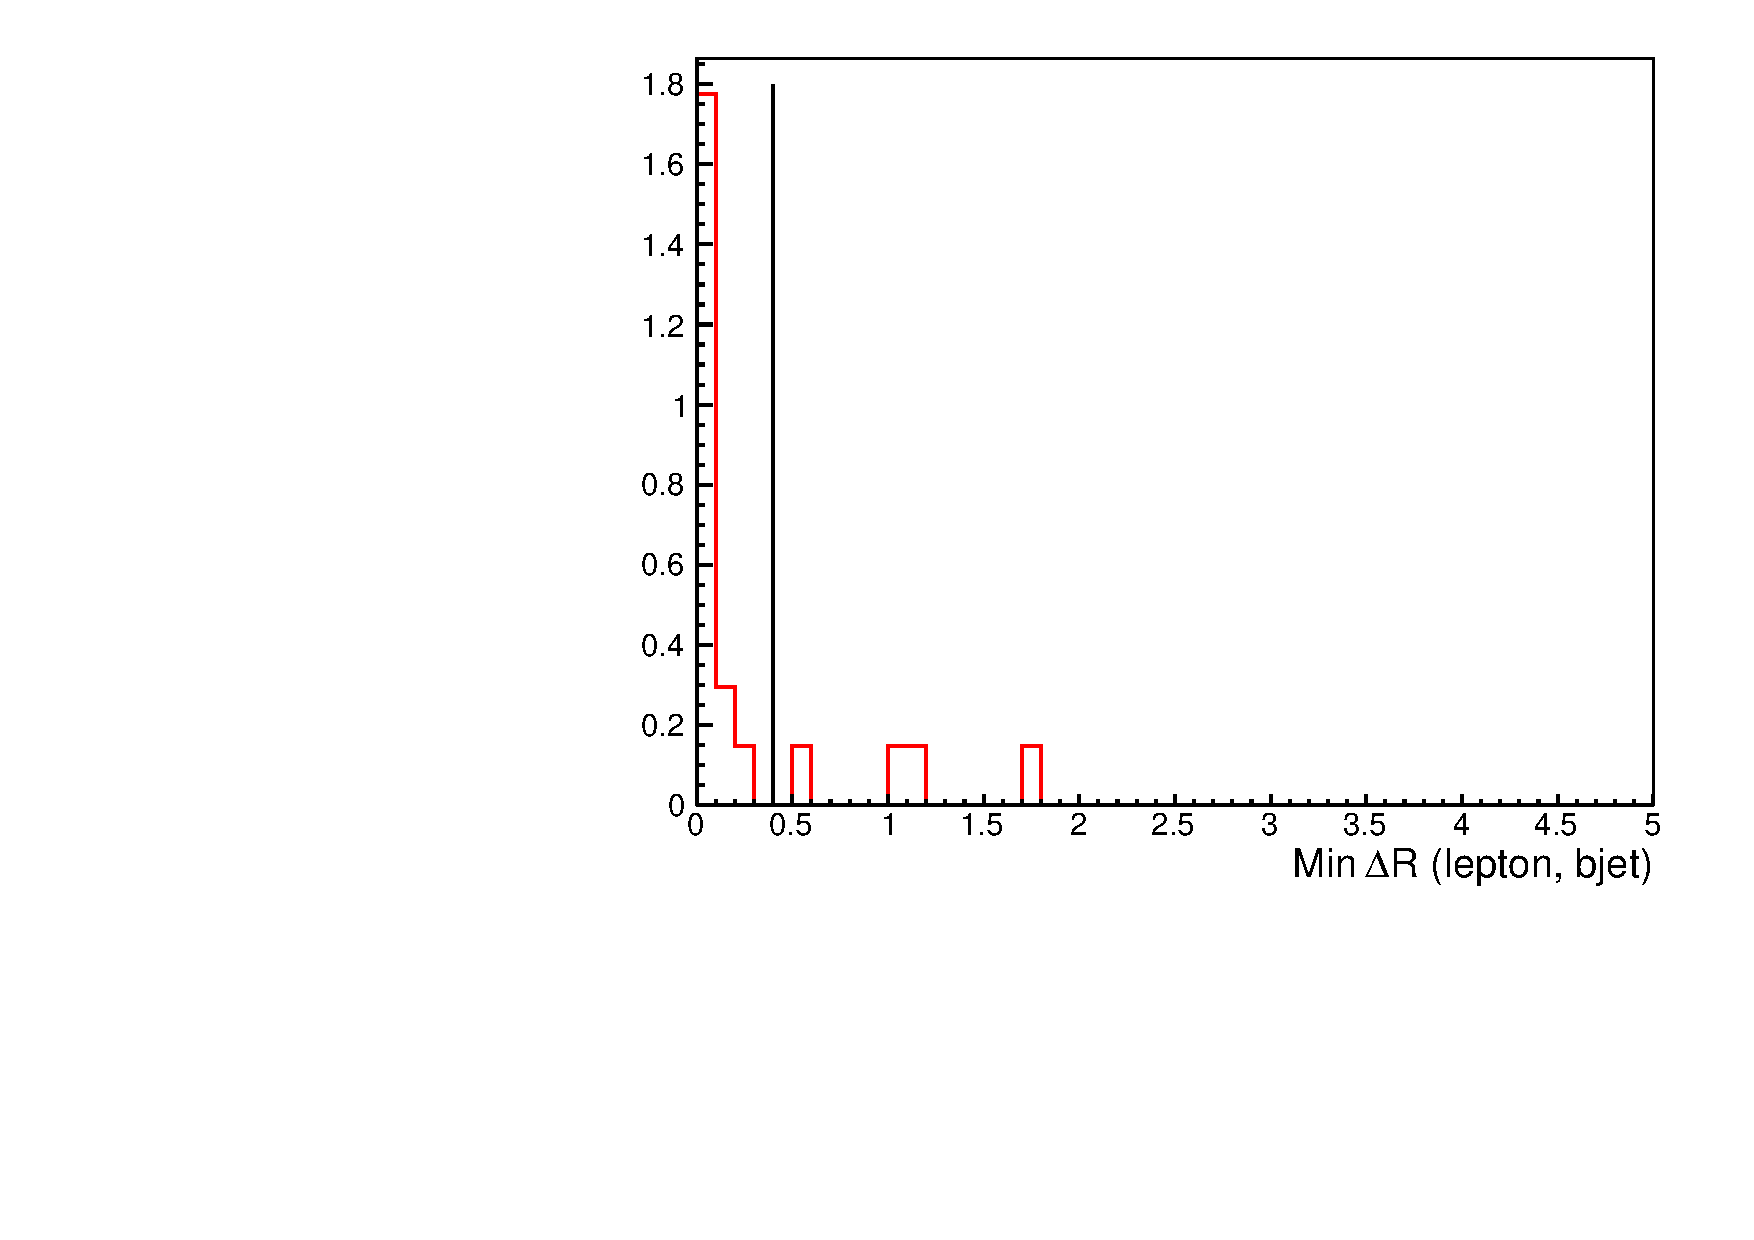
\includegraphics[width=0.6\linewidth, height=0.4\linewidth]{figs/bjetlepton.pdf}
\caption{ Minimum $\Delta R$ between the lepton and the b-tag jet in \ttbar\ decays.\label{fig:ttbar_residual}}
\end{center}
\end{figure}

Fig.~\ref{fig:ttbar_residual} shows that the bulk of such events in \ttbar\ decays are well within the $\Delta R < 0.4$ between lepton and the b-jet.



 




